\appendix
\section{Appendix}
% You may include other additional sections here.

\subsection{Datasets Summary}
Table \ref{tab:dataset_statistics} shows the number of image-text pairs of each datasets used in different pre-training methods.
% This table summarizes the number of image-text pairs used in the pre-training of FILIP, CLIP and ALIGN:
\begin{table}[h]
\center
\caption{Number of image-text pairs used in the pre-training of FILIP, CLIP and ALIGN.}
\label{tab:dataset_statistics}
\begin{tabular}{ c|cccc|c|c } 
 \hline
\multirow{2}{*}{} & \multicolumn{4}{c|} { FILIP } & { CLIP } & { ALIGN } \\
& CC3M & CC12M & YFCC100M & FILIP300M & \citep{radford2021learning} & \citep{jia2021scaling} \\ 
  \hline
 \# & 3M & 10M & 26M & 300M & 400M & 1800M \\
 \hline
\end{tabular}
\end{table}




\subsection{Detailed Experimental Settings}
\label{apdx:expt_setting}
%\footnote{better organize parts of diff tasks according to the order they appear in the main context.}


\begin{table}[htbp]
\caption{The architecture parameters for FILIP models.}
\label{tab:Filip_model_Hyperparameter}
    \centering
    % \resizebox{\textwidth}{!}{
    \begin{tabular}{l|cc ccc ccc}
        \toprule 
        \multirow{2}{*}{ Model } & Embedding & Input & \multicolumn{3}{c}{ Image Encoder } & \multicolumn{3}{c}{ Text Encoder } \\
          & dimension & resolution & \#layers & width & \#heads & \#layers & width & \#heads \\
        \midrule 
        
        $\text{FILIP}_{\text{base}}$  &  256 & $224\times 224$ & 12 & 768 & 12 & 12 & 512 & 8 \\
        $\text{FILIP}_{\text{large}}$ &  256 & $224\times 224$ & 24 & 1024 & 16 & 12 & 768 & 12 \\
        % $\text{FILIP}_{large+}$&  768 & 336 & 24 & 1024 & 16 & 12 & 768 & 12 \\
        \bottomrule
    \end{tabular}
    % }
\end{table}


\paragraph{Model Architectures.} 
We follow the same architecture design as CLIP, for both $\text{FILIP}_{\text{base}}$ and $\text{FILIP}_{\text{large}}$, except that we reduce the embedding dimension from 512/768 to 256 for the efficiency of loss computation.
Table \ref{tab:Filip_model_Hyperparameter} describes the details of architectures.

\begin{table}
    \centering
    \caption{Common hyperparameters used for FILIP pre-training.}
    % for common hyperparameters.}
    \label{tab:pre-training hyperparams}
    \centering
     \begin{tabular}{l|c}
        \toprule Hyperparameter & Value \\
        \midrule
        Vocabulary size & 49408 \\
        Initial temperature & $0.07$ \\
        LAMB $\beta_{1}$ & $0.9$ \\
        LAMB $\beta_{2}$ & $0.999$ \\
        LAMB $\epsilon$  & $10^{-4}$ \\
        Warm-up iters & 3000 \\
        Training epochs & 30  \\
        \bottomrule
    \end{tabular}
 
    \end{table}
  
\begin{table}
    \centering
    \caption{Model- and dataset-specific hyperparameters used for FILIP pre-training.
    % for model-specific and dataset-specific hyperparameters. 
    Numbers in batch size represent the total batch size across all workers and are calculated as: batch size per GPU $\times$ \#GPUs. FILIP340M is the combination of FILIP300M, YFCC100M, CC12M and CC3M.}
    \label{tab:Model_and_dataset_specific hyperparameters}
    \begin{minipage}{\textwidth}
        \centering
          \begin{tabular}{l|l|cccc}
        \toprule 
        Model  & Dataset  & Batch size & Base LR & Weight decay &  \\
        \midrule 
        $\text{FILIP}_{\text{base}}$ & YFCC100M & $1024 \times 8 $  & $6 \times 10^{-3}$ & 3e-2 \\
        $\text{FILIP}_{\text{base}}$  & FILIP340M & $ 320 \times 128 $ & $ 2 \times 10^{-3}$ & 3e-3  \\
        \midrule
        $\text{FILIP}_{\text{large}}$ & FILIP340M & $ 160 \times 192 $ &  $ 8 \times 10^{-4}$ & 3e-3  \\ 
        
        % \multirow{2}{*}{$\text{FILIP}_{large+}$} & YFCC100M   & $2 \times 10^{-5}$ & 3e-3 & 2000 \\
                                                % &  FILIP350M & $2 \times 10^{-5}$ & 3e-3 & 2000 \\
        % $\text{FILIP}_{large}$ & $4 \times 10^{-4}$ & 3e-3 & 768 & 224 & 24 & 1024 & 16 & 12 & 768 & 12 \\
        % $\text{FILIP}_{large+}$ & $2 \times 10^{-5}$ & 3e-3 & 768 & 336 & 24 & 1024 & 16 & 12 & 768 & 12 \\
        \bottomrule
    \end{tabular}
    \end{minipage}
\end{table}


\paragraph{Details for Pre-training and Hyperparameters.}  
For the implementation of the contrastive loss, following CLIP \citep{radford2021learning} and ALIGN \citep{jia2021scaling}, we also set the temperature in the softmax function to be a learnable parameter and initialize it as 0.07. 
For the pre-training, we use the LAMB optimizer implemented by the cybertronai's open-source repository (\url{https://github.com/cybertronai/pytorch-lamb}). 
For the learning rate scheduler, we first assign a base learning rate and then linearly warm it up to the peak learning rate according to the effective total batch size by a square root strategy, $peak\_lr=base\_lr \times \sqrt{\frac{total\_bs}{512}}$. 
We note that a large weight decay is crucial to stabilize training and improve generalization.
Specifically, we found that the training stability is a challenging issue when applying mix-precision training to large-scale models, i.e.,  the training is extremely unstable and the NaN loss easily happens. Recent works DALL-E \citep{ramesh2021zeroshot} and Cogview \citep{ding2021cogview} also notice this issue and provide their solutions. 
However, we found that simply increasing the weight decay and applying the trick of removing the weight decay of specific parameters as described in Section \ref{sec:experiment_details} work for our case.
The base learning rate and weight decay are selected manually via observing the performance at the early training stage.
Table \ref{tab:pre-training hyperparams} summarizes the common hyperparameters  and Table \ref{tab:Model_and_dataset_specific hyperparameters} shows the model- and dataset-specific hyperparameters for FILIP pre-training.


% \paragraph{Details for image captioning.} 
% \ylw{describe task setting. experimental details and training hyperparameters.}

% \begin{table}[htbp]
%     \centering
%     \caption{Hyperparameters used for image caption fine-tuning.}
%     \label{tab:hyperparameter_caption}
%     \begin{tabular}{l|cc}
%         \toprule Hyperparameter & cross-entropy optimization & CIDEr optimization \\
%         \midrule
%         batch size & 512 & 64\\
%         Training epochs & 30 & 5 \\
%         Optimizer & LAMB & AdamW \\ 
%         Learning rate & $3 \times 10^{-3}$ & $1 \times 10^{-5}$\\
%         Weight decay & $1 \times 10^{-4}$ & $1 \times 10^{-4}$\\
%         \bottomrule
%     \end{tabular}
% \end{table}


\paragraph{Details for Image-text Retrieval.} Following previous works \citep{jia2021scaling,li2021align}, for Flickr30K, we test on the 1K test set with or without fine-tuning on the 30K training set, while for MSCOCO, we test on the 5K test set with or without fine-tuning on the 113K training set.  We use the similarity between image and text for ranking and use the contrastive loss for fine-tuning. Since there are multiple texts for each image in these two datasets, we change the ground-truth label of contrastive loss to consider multiple positives, by assigning a probability of 1/\#positive to each positive following ALBEF~\citep{li2021align}. Besides, we also use prompts during evaluation for both datasets, see Appendix \ref{apdx:prompt_template} for details. Table \ref{tab:hyperparameter_image_text_retrieval} shows the hyperparameters for image-text retrieval fine-tuning.

\begin{table}[htbp]
    \centering
    \caption{Hyperparameters used for image-text retrieval fine-tuning.}
    \label{tab:hyperparameter_image_text_retrieval}
    \begin{tabular}{l|c}
        \toprule Hyperparameter & Value \\
        \midrule
        Image size & 392 $\times$ 392 \\
        Training epochs & 3 \\
        Optimizer & LAMB \\ 
        Batch size & 5120 \\
        Base LR & $2 \times 10^{-4}$ \\
        Weight decay & $3 \times 10^{-4}$ \\
        \bottomrule
    \end{tabular}
\end{table}


\subsection{More visualizations of Word-patch Alignment and Grad-cam Heatmaps}
\label{apdx:more_vis}
In Figure~\ref{fig:MoreImageNetVis}, we visualize the cross-modal alignment of the proposed method for more images, in terms of
both word-patch alignment as described in Section~\ref{sec:Visualization of Fine-grained Alignment} and Grad-CAM heatmaps~\citep{selvaraju2017grad}.
We compute the Grad-CAM heatmaps based on the average self-attention maps over the image patches classified to targeted textual tokens (i.e., the textual token(s) corresponding to the class label in the ImageNet dataset) in the last layer of the image encoder. We average the heatmaps over all attention heads.
As can be seen, our proposed model learns meaningful alignment between image patches and textual tokens.


\begin{figure}
\begin{center}
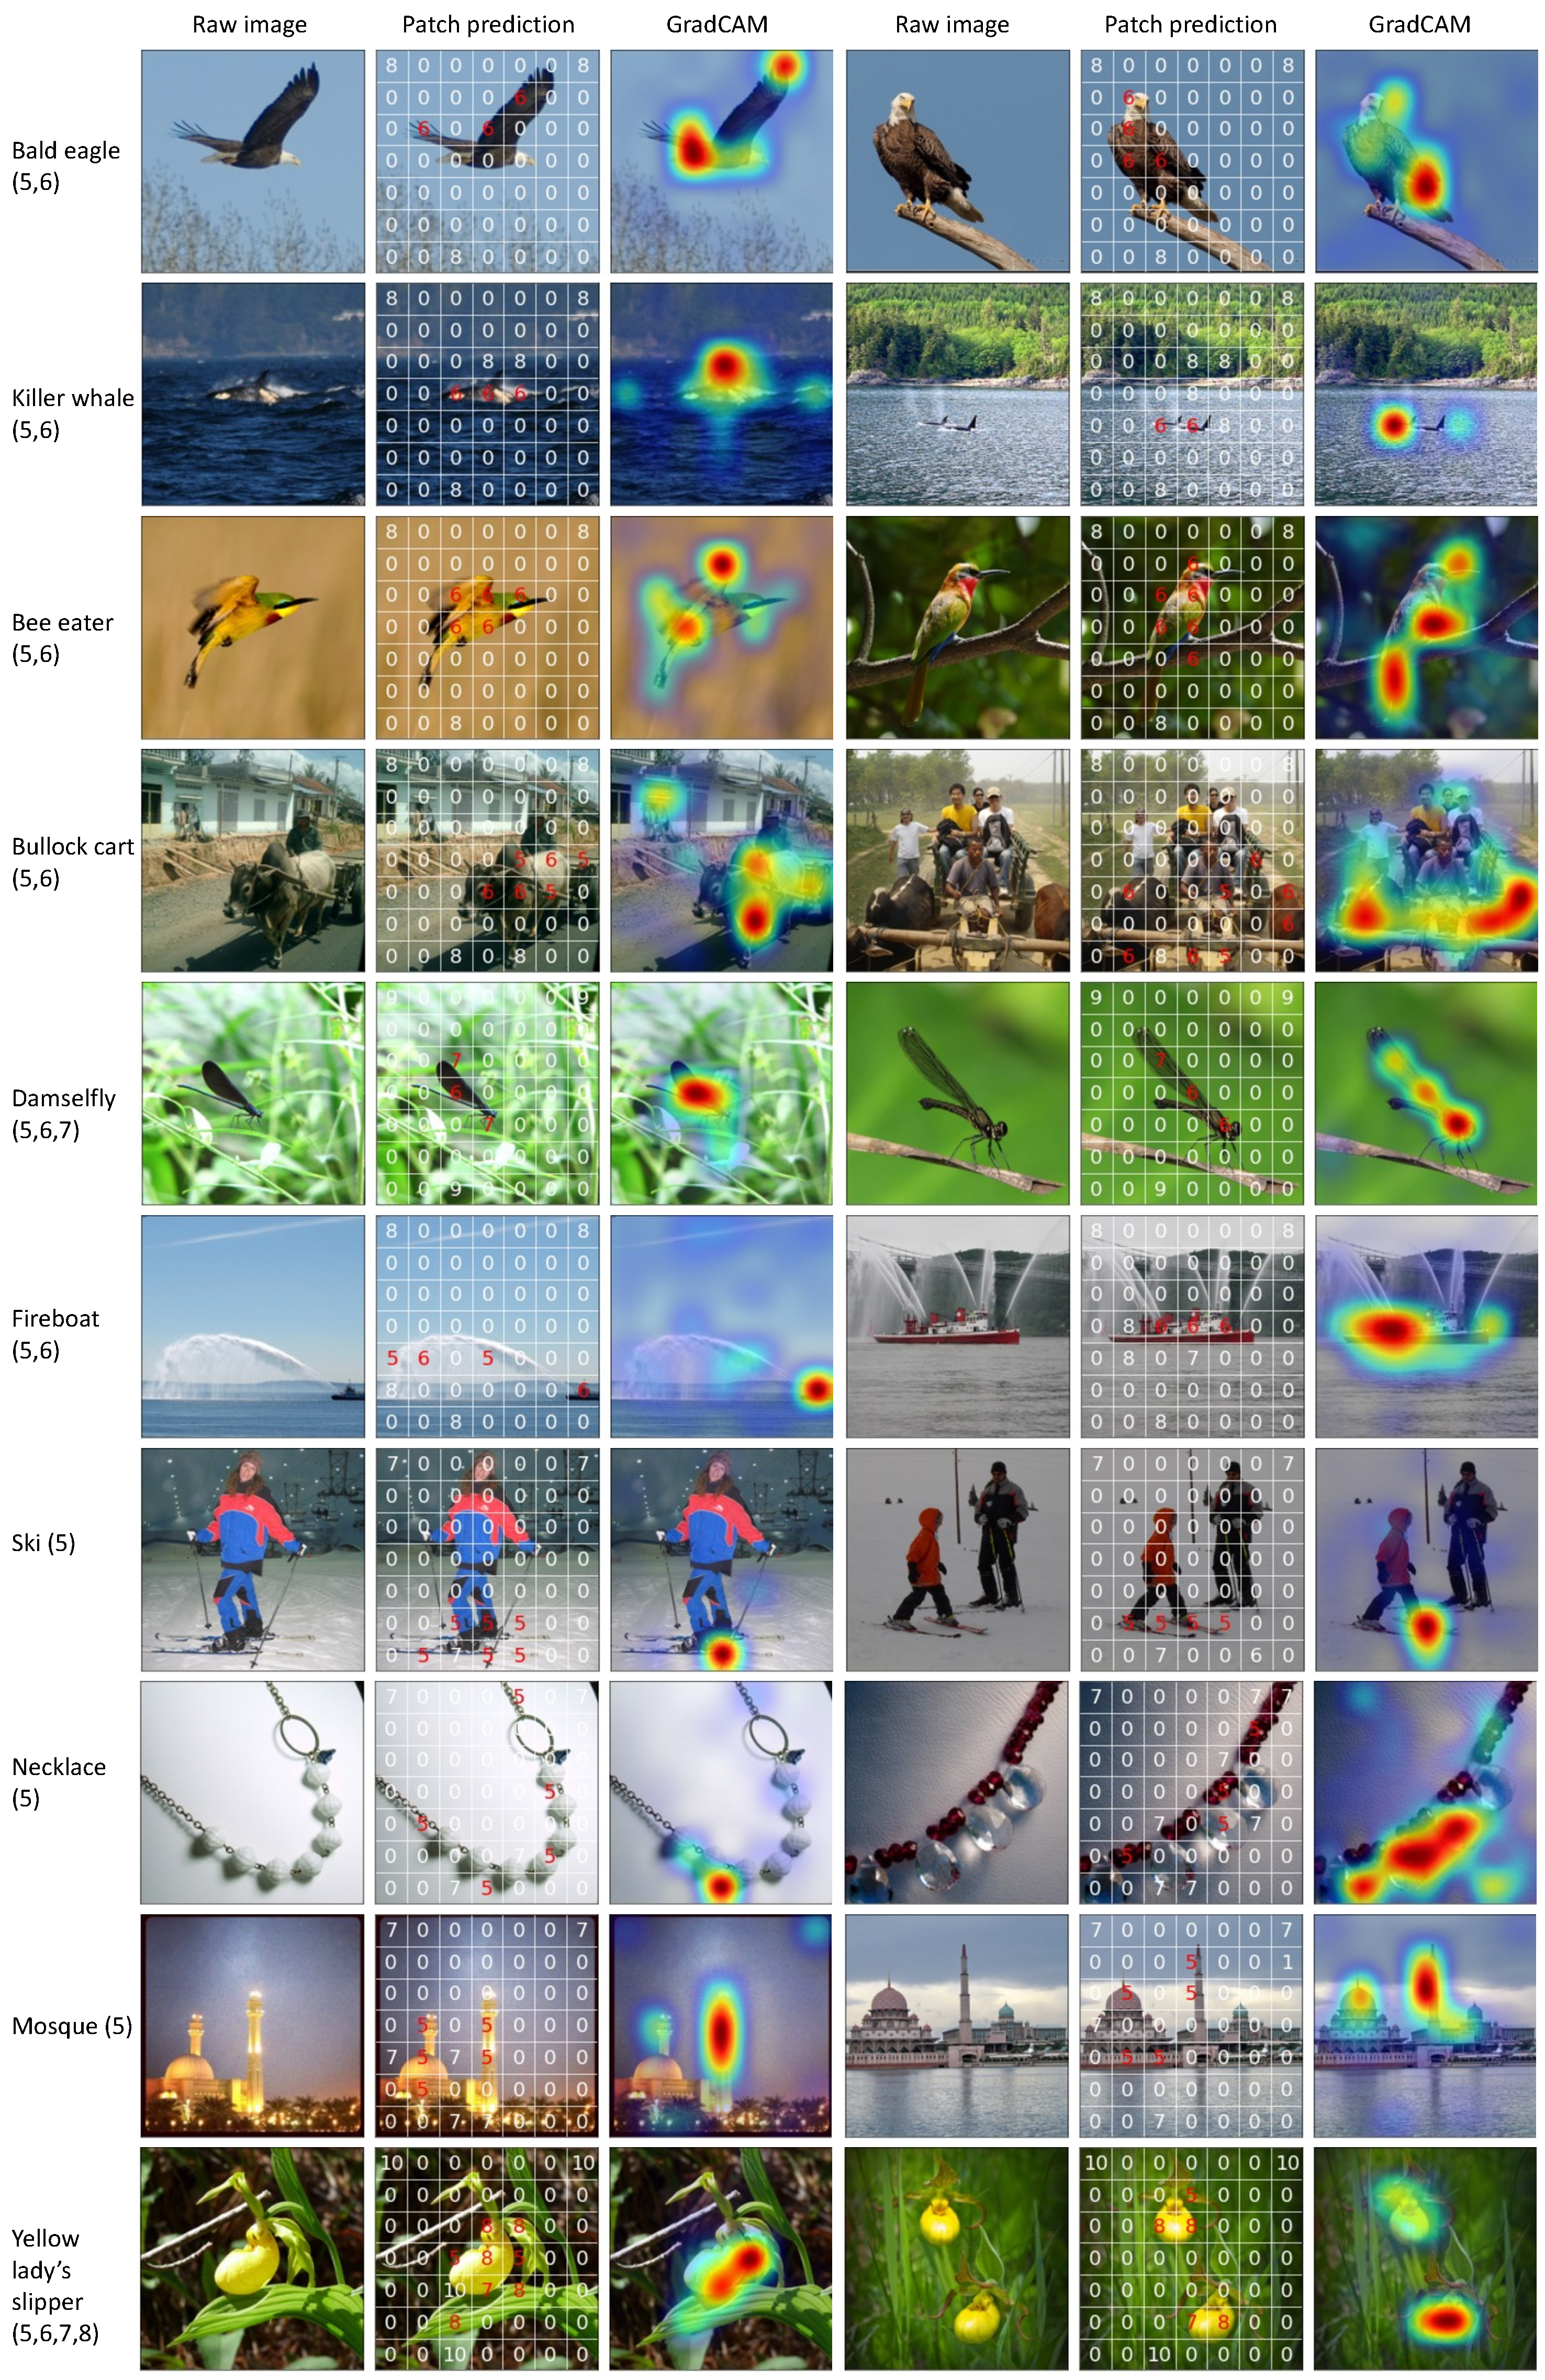
\includegraphics[width=\textwidth]{figures/ImageNetVis_appendix.pdf}
\caption{More visualizations on different classes of ImageNet dataset. Numbers in the parentheses after the class label indicate the location indices of class label in the tokenized textual sequence. }
\label{fig:MoreImageNetVis}
\end{center}
\end{figure}


\subsection{Prompt Templates for downstream tasks}
\label{apdx:prompt_template}
\paragraph{Image Classification.} Table~\ref{tbl:prompt_templates} shows the prompt templates for different image classification datasets
in the form of ``
$
\text{[prefix] \{label\}, [category description]. [suffix].} 
$
''
in Equation (\ref{eq:prompt_template}).
There are three components to be determined in the template, i.e., the prefix, the category description and the suffix.
For each component, we select several well-performed ones  for each dataset. 
Then we use the full combinations of all three components as the set of prompt templates for ensemble.
For instance, we use 5 prefixes, no category descriptions, and 6 suffixes for dataset ImageNet. 
Then the total number of prompt templates for this dataset is: $5 \times 1 \times 6=30$.

\paragraph{Image-text Retrieval.}  Following CLIP \citep{radford2021learning}, we use prompt in zero-shot image-text retrieval for both Flickr30K and MSCOCO datasets.
The prompt is selected by the same rule as described in Section~\ref{sec:prompt_ensemble}, except that we do not use ``[category description]'' here. Table \ref{tab:prompts_for_retrieval} shows the prompt templates for zero-shot image-text retrieval on Flickr30K and MSCOCO datasets. 


\begin{table}
\small
    \centering
    \caption{Prompt templates used for 12 downstream image classification tasks. 
    }
    \label{tbl:prompt_templates}
    \resizebox{\textwidth}{!}{
    \begin{tabular}{m{1.5cm}|m{4cm}|m{2cm}|m{4cm}}
    	\toprule
    	Dataset      & Prefix                                                                                                                                           & Category description                                             & Suffix                                                                                                                                                \\ \midrule
    	CIFAR10      & ``a photo of a", ``a jpeg photo of a", ``a painting of a", ``itap of a", ``graffiti of a", ``a cartoon", ``a doodle"                                                      & None                                                             & None, ``It's common in daily life", ``It's cute", ``It's ugly", ``It's weird", ``Hope you like it"                                                     \\ \midrule
    	CIFAR100     & ``a jpeg photo of a", ``a painting  of a", ``a good photo  of a", ``a bad photo  of a", ``a photo  of a", ``itap of a", ``a rendering  of a"                                              & None                                                             & None, ``It's common in daily life", ``It's beautiful", ``It's ugly", ``I like it", ``I take it today"                                                  \\ \midrule
    
    	Caltech101   & ``a photo  of a", ``a cropped photo  of a", ``a good photo  of a", ``a bad photo  of a"                                                                                  & None                                                             & None, ``I like it", ``I hate it", ``It's ugly", ``It's cute"                                                                                           \\ \midrule
    	Stanford-Car & ``a photo  of a", ``a close-up photo  of a", ``a good photo  of a", ``a bad photo  of a"                                                                                 & ``a type of car", ``a type of automobile"                        & ``I like it", ``It belongs to my friend", ``It's brand new", ``It's popular recently", ``It's important to me", ``I take it today"                    \\ \midrule
    	Flowers102   & ``a photo of a (many) ", ``a rendering of a (many) ", ``itap of a (many) "                                                                                                                & ``a type of flower", ``a type of bloom"                          & ``It's beautiful", ``It's from my best friend", ``It gives out a sweet perfume/fragrance"                                                             \\ \midrule
    	ImageNet       & ``a photo of a", "a good photo of a", ``a bad photo of a", ``a close-up photo of a", ``itap of a"                                                                         & None                                                             & ``I like it", ``It's common in daily life", ``It's not common in daily life", ``It's ugly", ``It's cute", ``It's beautiful"                           \\ \midrule
    	Food101      & ``a photo of my", ``a close-up photo  of my", ``itap  of my"                                                                                                         & ``a type of food", ``a type of nourishment"                      & ``I made it today", ``I like it", ``I hate it", ``It's delicious", ``It's with nice flavour", ``It's with terrible flavour", ``It's popular recently" \\ \midrule
    	SUN397       & ``a photo  of a", ``a good photo  of a", ``a bad photo  of a", ``a bright photo  of a", a dark photo  of a", ``a black and white photo  of a", ``a nice scene  of a", ``a terrible scene  of a" & None                                                             & None, ``I like it", ``I hate it", ``It's beautiful", ``It's common in daily life", ``It's important to me"                                             \\ \midrule
    	DTD          & ``itap of a", ``a close-up photo of a"                                                                                                                     & ``texture", ``surface", ``material"                              & None, ``It's out of style", ``It's popular in old days", ``It's ugly", ``It's beautiful"                                                               \\ \midrule
    	Aircrafts    & ``a photo of the", ``a close-up photo of the", ``a good photo of the ", ``a pixelated photo of the"                                                                           & ``a type of plane", ``a type of aircraft", ``a type of airliner" & None,``I like it", ``It's important to me", ``I take it today", ``Hope you like it"                                                                    \\ \midrule
    	Oxford Pet   & ``a photo of my", ``a low resolution photo of my", ``a good photo of my"                                                                                           & ``a type of pet", ``a type of dog or cat"                        & None, ``It's cute", ``It's important to me", ``I like it", ``It's beautiful"                                                                           \\ \midrule
    	EuroSAT      & ``a photo  of a", ``a painting of a", ``a cropped photo of a", ``a good photo of a", ``a blurry photo of a"                                                                 & None, ``an example of aerial or satellite images"                 & None, ``I like it", ``It's taken from an aircraft or some flying object", ``It's collected by imaging satellites"                                      \\ \bottomrule
    \end{tabular}
    }
\end{table}



\begin{table}[!t]
\small
    \centering
    \caption{Prompt templates used for zero-shot image-text retrieval on Flickr30K and MSCOCO datasets. 
    }
    \label{tab:prompts_for_retrieval}
    \resizebox{0.8\textwidth}{!}{
    \begin{tabular}{m{1.5cm}|m{3cm}|m{3cm}|m{1.5cm}}
    	\toprule
    	Dataset  & Task & Prefix  & Suffix \\ \midrule
    	\multirow{2}{*}{ Flickr30K } & image-to-text retrieval      & ``a good photo of the'' &  ``I hate it.''        \\ 
    	 & text-to-image retrieval      & ``a good photo of'' &  None        \\ \midrule
    	\multirow{2}{*}{ MSCOCO } & image-to-text retrieval      & ``a good photo of'' &  ``It is ugly.''        \\ 
    	 & text-to-image retrieval      & None &  None       \\ \bottomrule

    \end{tabular}
    }
\end{table}


% \begin{table}
%     \centering
%     \caption{Prompts used for 13 downstream image classification tasks. 
%     % \hou{In the template for each dataset, ``[pref]'' is short for ``Prefix'', ``\{\}'' denotes the class label. ``[des]'' is short for ``Category Description'', and ``[suff]'' is short for ``Suffix''.}
%     }
%     \label{tbl:prompt_templates}
%     \resizebox{\textwidth}{!}{
%     \begin{tabular}{m{1.5cm}|m{2cm}|m{4cm}|m{2cm}|m{4cm}}
%     \hline
%         Dataset & Template & Prefix & Category Description & Suffix \\ \hline
%         CIFAR10 & [pref] of a \{\}. [suff]. & "a photo", "a jpeg photo", "a painting", "itap", "graffiti", "a cartoon", "a doodle" & None & "", "It's common in daily life", "It's cute", "It's ugly", "It's weird", "Hope you like it" \\ \hline
%         CIFAR100 & [pref] of a \{\}. [suff]. & "a jpeg photo", "a painting", "a good photo", "a bad photo", "a photo", "itap", "a rendering" & None & "", "It's common in daily life", "It's beautiful", "It's ugly", "I like it", "I take it today" \\ \hline
%         CUB-Birds & [pref] of a \{\}, [des]. [suff]. & "a close-up photo", "itap" & "a type of bird", "a type of animal" & "It's common in daily life", "It's cute", "I like it" \\ \hline
%         Caltech101 & [pref] of a \{\}. [suff]. & "a photo", "a cropped photo", "a good photo", "a bad photo" & None & "", "I like it", "I hate it", "It's ugly", "It's cute" \\ \hline
%         Stanford-Car & [pref] of a \{\}, [des]. [suff]. & "a photo", "a close-up photo", "a good photo", "a bad photo" & "a type of car", "a type of automobile" & "I like it", "It belongs to my friend", "It's brand new", "It's popular recently", "It's important to me", "I take it today" \\ \hline
%         Flowers102 & [pref] of a (many) \{\}. [suff]. & "a photo", "a rendering", "itap" & "a type of flower", "a type of bloom" & "It's beautiful", "It's from my best friend", "It gives out a sweet perfume/fragrance" \\ \hline
%         ImageNet & [pref] of a \{\}. [suff]. & "a photo", "a good photo", "a bad photo", "a close-up photo", "itap" & None & "I like it", "It's common in daily life", "It's not common in daily life", "It's ugly", "It's cute", "It's beautiful" \\ \hline
%         Food101 & [pref] of my \{\}, [des]. [suff]. & "a photo", "a close-up photo", "itap" & "a type of food", "a type of nourishment" & "I made it today", "I like it", "I hate it", "It's delicious", "It's with nice flavour", "It's with terrible flavour", "It's popular recently" \\ \hline
%         SUN397 & [pref] of a \{\}. [suff]. & "a photo", "a good photo", "a bad photo", "a bright photo", "a dark photo", "a black and white photo", "a nice scene", "a terrible scene" & None & "", "I like it", "I hate it", "It's beautiful", "It's common in daily life", "It's important to me" \\ \hline
%         DTD & [pref] of a \{\} [des]. [suff]. & "itap", "a close-up photo" & "texture", "surface", "material" & "", "It's out of style", "It's popular in old days", "It's ugly", "It's beautiful" \\ \hline
%         Aircrafts & [pref] of the \{\}, [des]. [suff]. & "a photo", "a close-up photo", "a good photo", "a pixelated photo" & "a type of plane", "a type of aircraft", "a type of airliner" & "", "I like it", "It's important to me", "I take it today", "Hope you like it" \\ \hline
%         Oxford Pet & [pref] of my \{\}, [des]. [suff]. & "a photo", "a low resolution photo", "a good photo" & "a type of pet", "a type of dog or cat" & "", "It's cute", "It's important to me", "I like it", "It's beautiful" \\ \hline
%         EuroSAT & [pref] of a \{\}, [des]. [suff]. & "a photo", "a painting", "a cropped photo", "a good photo", "a blurry photo" & "", "an example of aerial or satellite images" & "", "I like it", "It's taken from an aircraft or some flying object", "It's collected by imaging satellites" \\ \hline
%     \end{tabular}
%     }
% \end{table}





